%%% -*-LaTeX-*-

\chapter{Results}

In this chapter we describe the results of our experiments so far and illustrate how they are a step towards our thesis goal.

\begin{itemize}
	\item We were able to extract different host behaviors of interest to network admin, here we are mentioning two of them, namely scanners and DNS Query Responses. The cluster that contains scanners have a high
	
	\item 
	We were able to extract different host behaviors of interest to network admin, here we are mentioning two of them, namely scanners and DNS Query Responses. The cluster that contains scanners have a high
\end{itemize}

\begin{itemize}
\item We were able to extract different host behaviors of interest to network admin, here we are mentioning two of them, namely scanners and DNS Query Responses. The cluster that contains scanners have a high incoming traffic trying to infiltrate the
network by scanning for open ports. The amount of packets and bytes transferred by hosts in this cluster is unsubstantial. The behavior exhibited by the hosts of this
cluster can be used by the network admin to monitor the security of the network.
The cluster that contains DNS Query Responses has heavy traffic aiming at a single
port. Studying about this cluster behavior over time will give an edge in planning
bandwidth of the network. The remarkable feature of our system is that it has extracted
the above behaviors without any prior knowledge of the hosts in the system or the input Netflow data.
\item We have observed that over periods of short intervals of time(few weeks), the number
of clusters have remained fairly constant which indicates that there has been no
rapid change in the behaviors exhibited by the hosts. And our system performed
seemingly well by choosing a constant number of clusters at the stage of pattern
detection. Figure \figref{constant} represents how the number of clusters formed for a months
data are close to constant.

\item  By mapping cluster behaviors of a given day with a reference day we were also able
to compare host behaviors. These comparisons can help network admin in capacity
planning, threat analysis and other network monitoring activities. We built a tool to analyze these host behaviors. 
We provide network admin with an option to compare
behaviors on two days as shown in figure \figref{compare_days}


\end{itemize}

\begin{figure}[t]
	\centerline{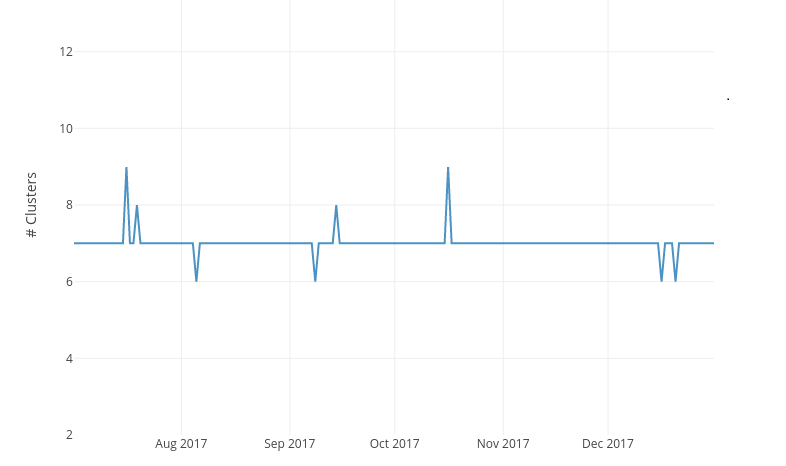
\includegraphics{constant.png}}
	\caption{ Plot of number of clusters formed over a time period.}%
	\figlabel{constant}
\end{figure} 

\begin{figure}[t]
	\centerline{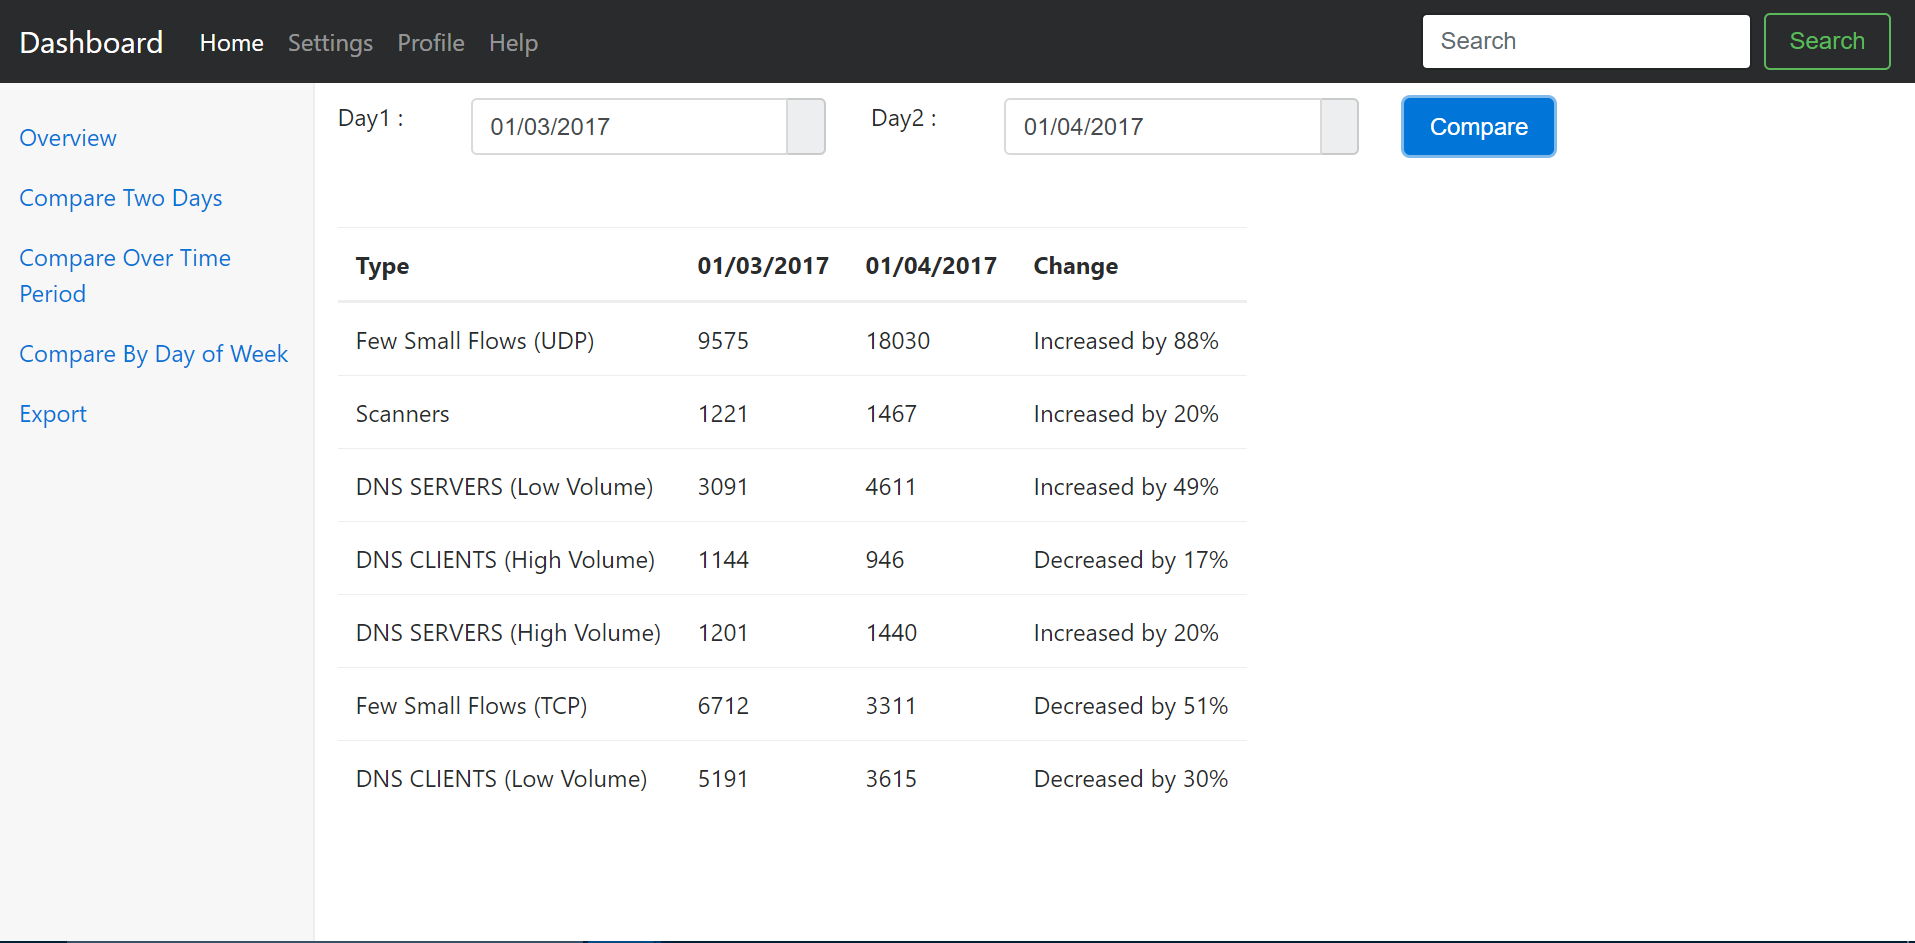
\includegraphics[scale = 0.45]{tool_compare_days.png}}
	\caption{Compare Host Behaviors on two days.}%
	\figlabel{compare_days}
\end{figure} 

The figure \figref{compare_weeks} gives an insight of how hosts behavior is changing over a month.
In the graph each line represents different host behaviors. The X-axis and Y-axis
represent the date on which this host behavior is observed and the number of hosts
which exhibited this behavior respectively.

\begin{figure}[t]
	\centerline{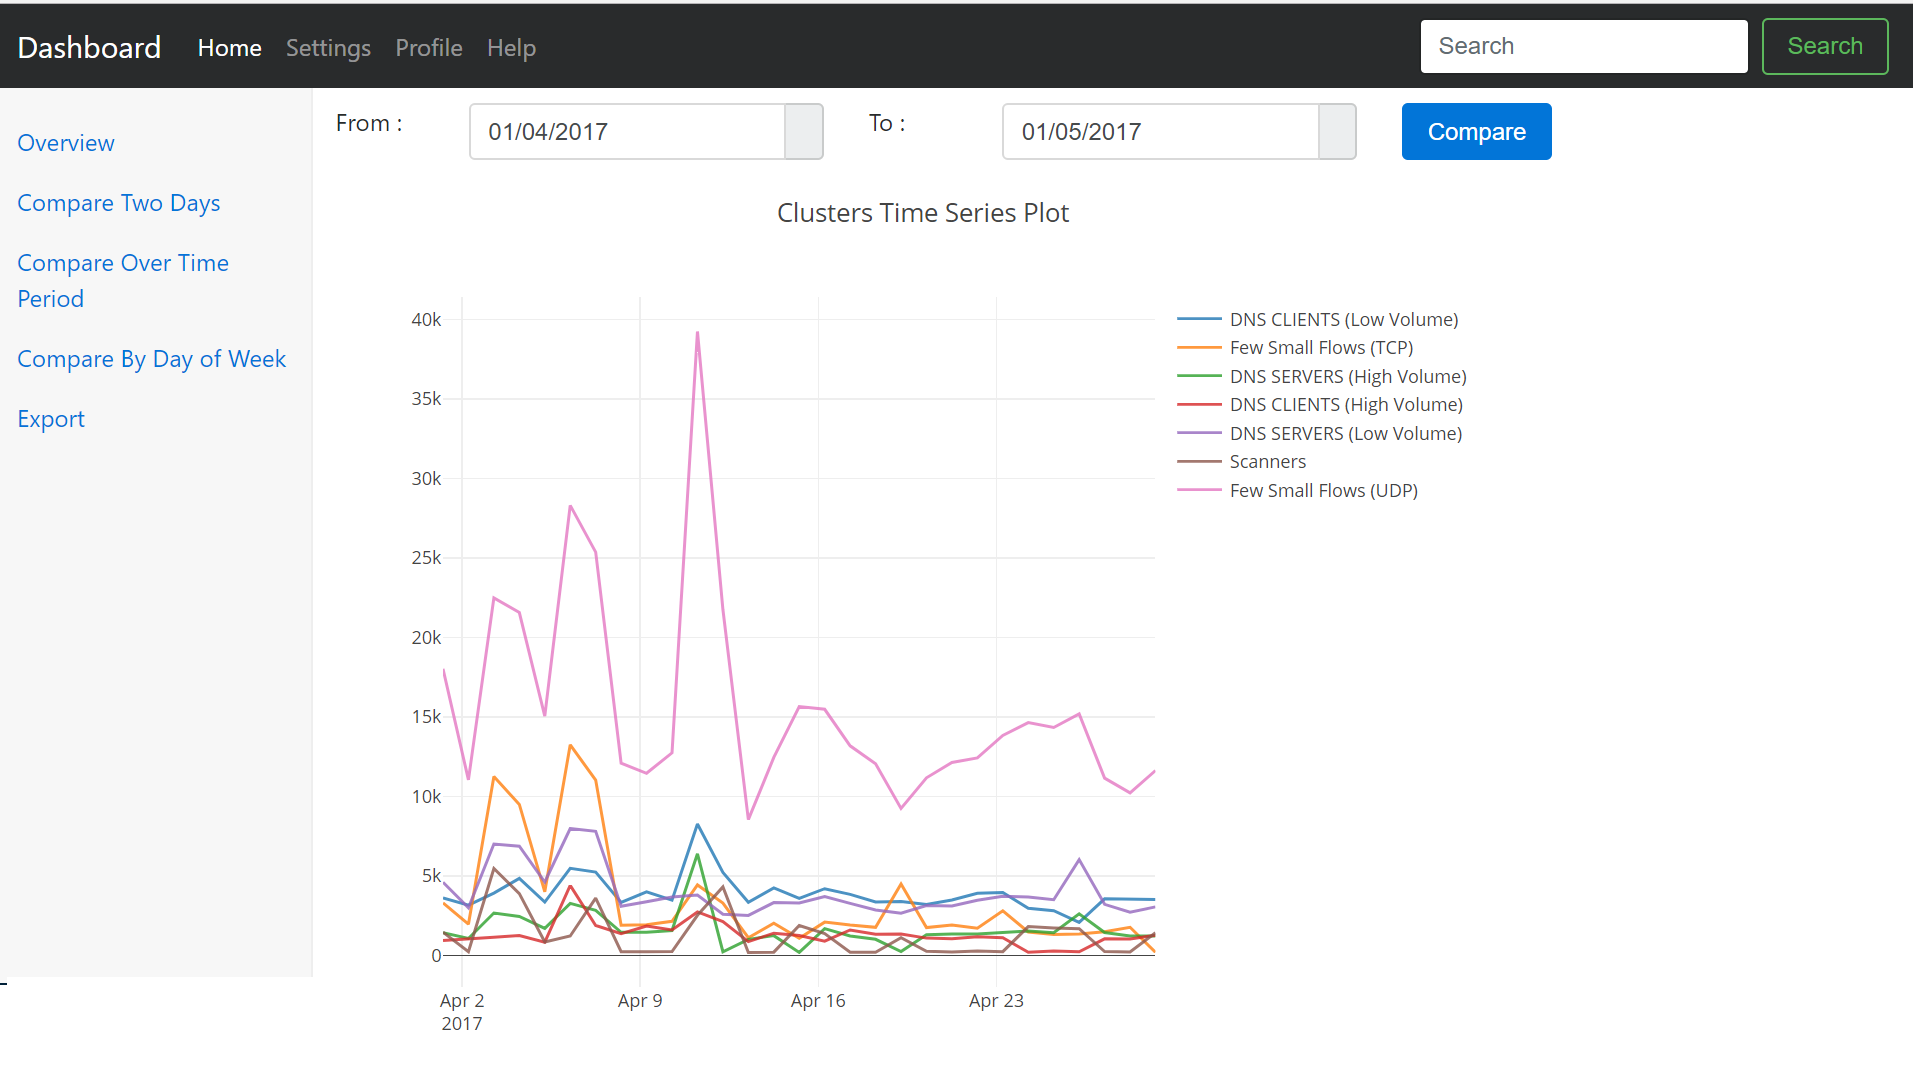
\includegraphics[scale = 0.45]{tool_compare_week.png}}
	\caption{Compare Host Behaviors over a time period.}%
	\figlabel{compare_weeks}
\end{figure} 



\section{Evaluation}

\tabref{evaluation} shows the planned evaluations of our sytsem which will be included in the final thesis defense.

\begin{table}[b]
		\caption{Planned Evaluations}%
	\centerline{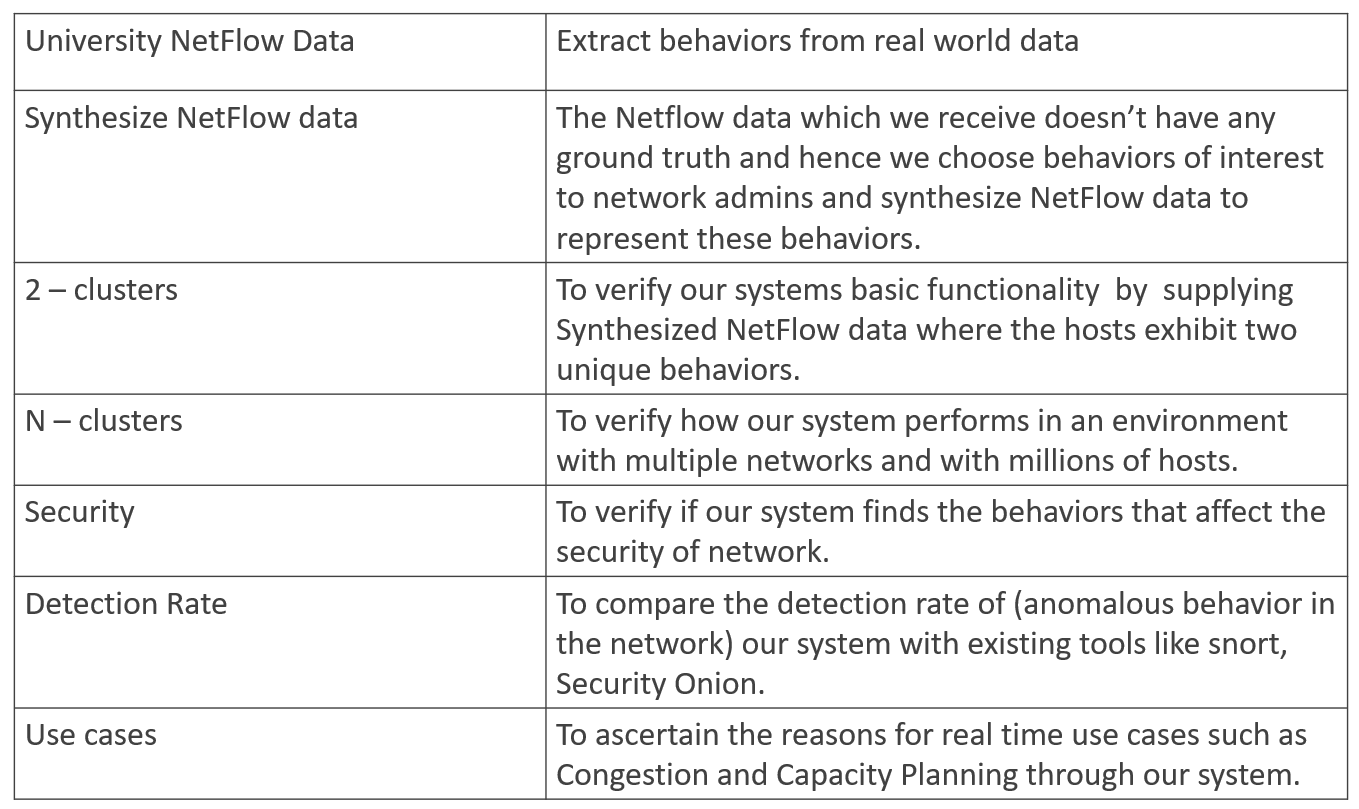
\includegraphics[scale = 0.6]{evaluation.png}}
	\tablabel{evaluation}
\end{table}


As Netflow data is unlabeled it gets tough to test few functionalities of the system
that we have built. Hence, in order to overcome this we want to insert some behaviors
into the NetFlow data(create simulated environment) and verify if our system is able to
detect them. Even with simulated environment one has to remember that we are not going
to provide any information pertaining to the behaviors of the hosts of the system or the
simulated data yet our system is expected to uncover them. In addition to this we will also
present set of results using real data.




The two main functionalities that we would like to test are :
\begin{itemize}
	
	\item Detecting the anomalous hosts in the network through host behaviors and find other
	such hosts that are of interest to security of network.
	
	\item Helping network administrator to efficiently predict the capacity needs of the network.
\end{itemize}

We would like to create a micro benchmark using the existing NetFlow analysis tools
for both the above scenarios. For the first scenario, we synthesize flow data that has
scanners trying to enter the system along with the web traffic(Http requests, DNS requests
and others..) and pass it through the existing tools. We expect these tools to give a detailed
sketch about the traffic based on applications and ports. But, when the same traffic is
passed through our system the expected output is at least two clusters one with normal
web traffic and the other with scanners. This is the important point that we would like to
mention about our system that is it extracts the information that we have never asked it to
look for.
Before talking about the second scenario, let us see how the state-of-art network analysis
tools perform bandwidth management. Solarwinds is an organization that provides
Network Management softwares. One of it’s licensed products is ”Netflow Traffic Analyzer
and Bandwidth monitoring software”. This tool works with Cisco NetFlow, Juniper
J-Flow, sFlow, Huawei NetStream, and IPFIX flow data and monitors bandwidth use by
application, protocol, and IP address group and identifies which applications, and protocols
are consuming the most bandwidth. So,our benchmark for second scenario would be
to synthesize flow data which needs more than an aggregation on application or protocol
to determine capacity needed for network and pass it through open source tools that use
similar bandwidth management techniques as Solarwinds. Similarly, on the other hand
we pass this data through our system and our expectation would be that we will be find
few clusters that will help admin understand which hosts are consuming the network
bandwidth and take suitable actions.